\noindent
Spadek gradientowy jest to jeden ze sposobów odnalezienia najlepszej regresji. Używa on do tego funkcję kosztu, do której parametry modyfikuje sobie w zależności od kroku ($\alpha$) oraz pochodnej po kierunku. Wzór na spadek gradientowy powtarzamy aż do otrzymania wszystkich pochodnych równych 0 lub określoną ilość iteracji.
\large
$$
\theta_{j} := \theta_{j} - \alpha \frac{\partial}{\partial\theta_{j}} J(\theta_{0}, \theta_{1})
$$
\normalsize
\noindent
\newline
W zależności od ilości $\theta$ będziemy musieli równocześnie aktualizować tyle nowych $\theta$. Wzór jest w pewnym sensie uproszczeniem, tak naprawdę po lewej stronie nie będą stały $\theta_{j}$, a $\theta_{j}temp$, a na samym końcu wszystkie $\theta$ będą uaktualniane. 


	\begin{figure}[H]
    \centering
    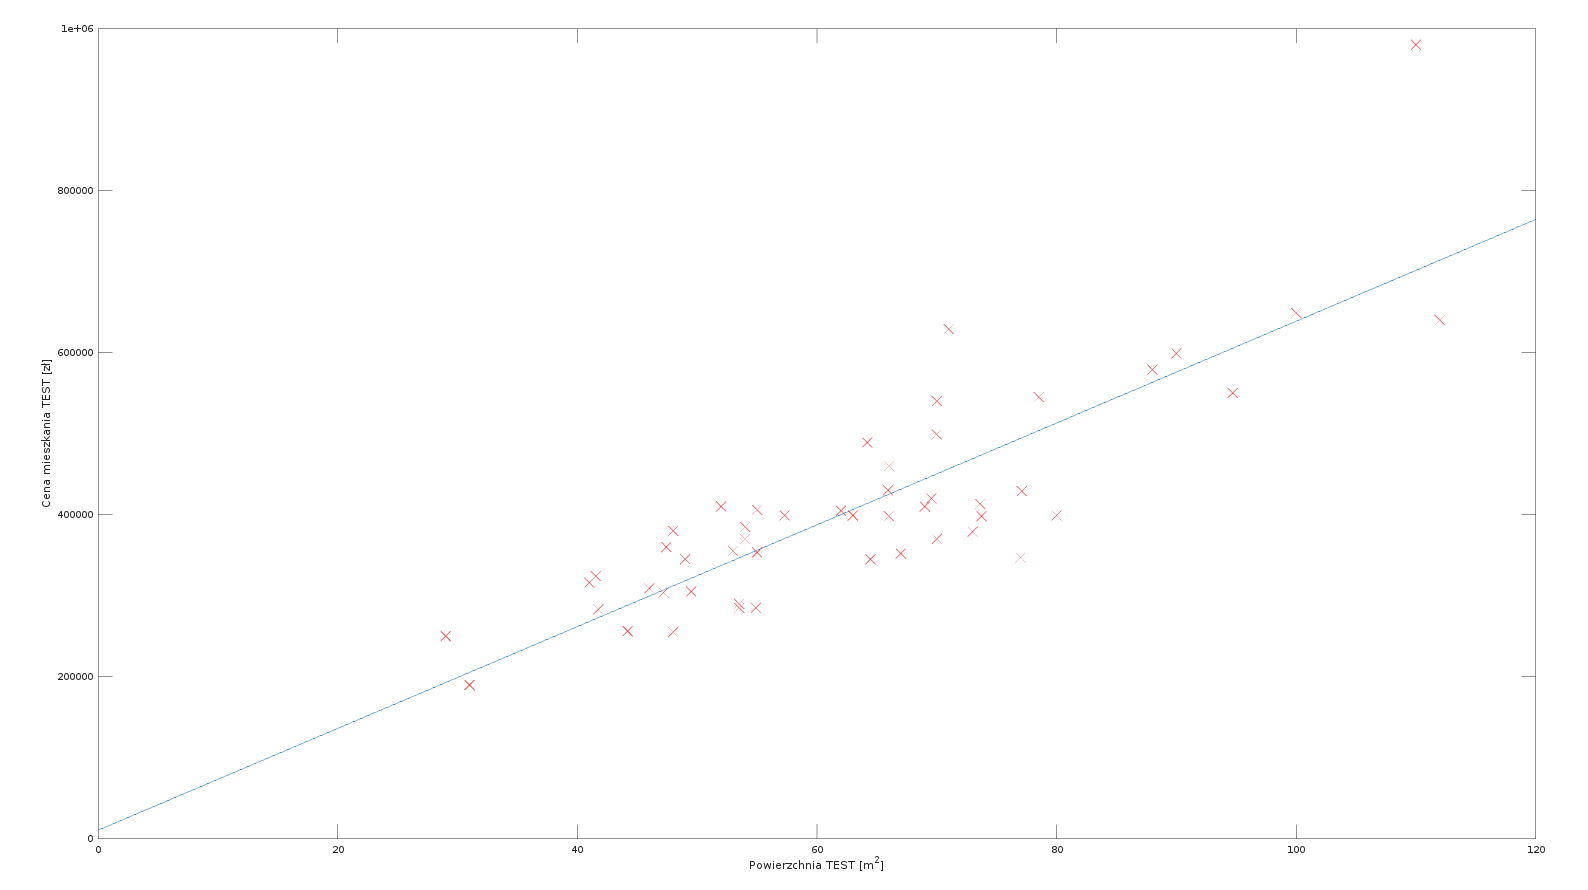
\includegraphics[scale=0.22]{PNG/perfect_grad.png}
    \caption{Idealna regresje znaleziona przez spadek gradientowy}
    \label{lamana}
	\end{figure}
	

Powyższy wykres pokazuje znalezioną funkcje kosztu - nie istnieje inna funkcja kosztów z innymi parametrami, która lepiej opisałaby te dane. W takim razie można powiedziec, że nie zostało tylko osiągnięte lokalne ekstremum, a nawet globalne minimum.

\newpage

Jak w takim razie wygląda dokładnie algorytm spadku gradientowego? Po pierwsze nasz algorytm trwa określoną ilość iteracji. W pierwszym momencie można pomyśleć, że kończy się zbyt wcześnie i nie dochodzi do minium, aczkolwiek praca nad nim polega właśnie na dopasowaniu parametrów - kroku spadku oraz ilości iteracji.

\begin{verbatim}
	   for iteracja = 1 : ilosc_iteracji
	      h = X * theta
	      theta = theta - alpha * (1/m) * (X' * (h - y))
	   end
\end{verbatim}

Jak widać mimo całej złozoności problemu sam algorytm jest bardzo prosty. Wcześniej wspominaliśmy o tym, że trzeba sprawdzić czy algorytm na pewno znajduje minimum. Można to zrobić rysując zależność funkcji kosztu od poszczególnych theta. Nie jesteśmy w stanie narysować pełnej funkcji, ale dzięki zachowaniu parametrów takich jak historyczne dane J oraz $\theta$. Jeżeli widać, że dla naszego wykresu w pewnym momencie J jest stałe oznacza to, że doszliśmy do momentu, gdy osiągneliśmy szukane przez nas $\theta_{0}$ oraz $\theta_{1}$.
\newline
\newline
\noindent
Kied w takim razie kończy się spadek gradientowy? Dzięki matematyce wiemy, że minimum jest to miejsce, w którym osiągamy najniżej połozony punkt, czyli przed i po w każdym kierunku powinniśmy posiadać wartości większe. Dzięki pochodnej wiemy czy to jest ten punkt, ponieważ pochodne po każdym kierunku powinny wynosić 0.